\documentclass{TDP005mall}



\newcommand{\version}{Version 1.1}
\author{Niklas Åsberg, \url{nikas214@student.liu.se}}
\title{Kravspecification}
\date{2023-11-24}
\rhead{Niklas Åsberg}
\usepackage{graphicx}
\graphicspath{{./}}


\begin{document}
\projectpage
\section{Revisionshistorik}
\begin{table}[!h]
\begin{tabularx}{\linewidth}{|l|X|l|}
\hline
Ver. & Revisionsbeskrivning & Datum \\\hline
0.1 & Utkast & 2023-11-12 \\\hline
1.0 & Utökat antal krav och förtydligat beskrivningen & 2023-11-18 \\\hline
1.1 & Ändringar efter feedback & 2023-11-24 \\\hline
\end{tabularx}
\end{table}

\tableofcontents
\newpage

\section{Spelidé}
Spelet är ett tvådimentionellt arkadspel, målet är att ta sig igenom så många labyrinter som möjligt på så kort tid som möjligt utan att dö.
Spelplanen är ett rutnät, all förflyttning sker mellan rutor intill varandra. Det kommer finnas väggar på vissa rutor som man inte kan röra sig igenom.
Det kommer vara massa fiender ivägen för spelaren som spelaren ska ta sig förbi eller förinta. 
Fiender kan skada spelaren om de hamnar i samma ruta, hur mycket skada spearen tar är olika beroende på fiende-typ.
Spelaren kan attackera fiender när fienderna är en ruta bort.
Målgruppen för spelet är de som gillar arkadspel och speed-runners.
Spelet har mycket fokus på snabbhet, så spelaren kommer att försöka slå sin bästa tid och tävla med andra spelara om vem som får högst poäng.

\section{Spelmekanik}
Man styr sin spelare med W, A, S och D tangenterna och attackerar med mellanslag. Varje bana är en labyrint när spelaren ska ta sig till utgången, när spelaren tagit sig till utgången så börjar nästa bana.
Det finns fiender som är i vägen och dessa kommer att skada spelaren om de är på samma ruta.
Spelaren behöver inte nödvändigtvis förinta fienderna för att klara banan men spelaren får extrapoäng om spelaren förintar fiender.

\section{Regler}
Varken spelaren eller fiender kan röra sig till en ruta där det finns en vägg.
Spelaren tar skada om spelaren befinner sig på samma ruta som en fiende.
Spelaren kan skada en fiende som står en ruta framför spelaren genom att attackera.
När spelaren är på rutan där utgången finns så är banan avklarad och spelaren flyttas till nästa bana.
Om spelaren inte har några livspoäng kvar så börjar spelet om.
Spelaren "Vinner" genom att ta sig igenom alla banor.

\newpage
\section{Visualisering}
Spelet kommer vara tvådimentionellt och vara ur ett fågelperspektiv. 

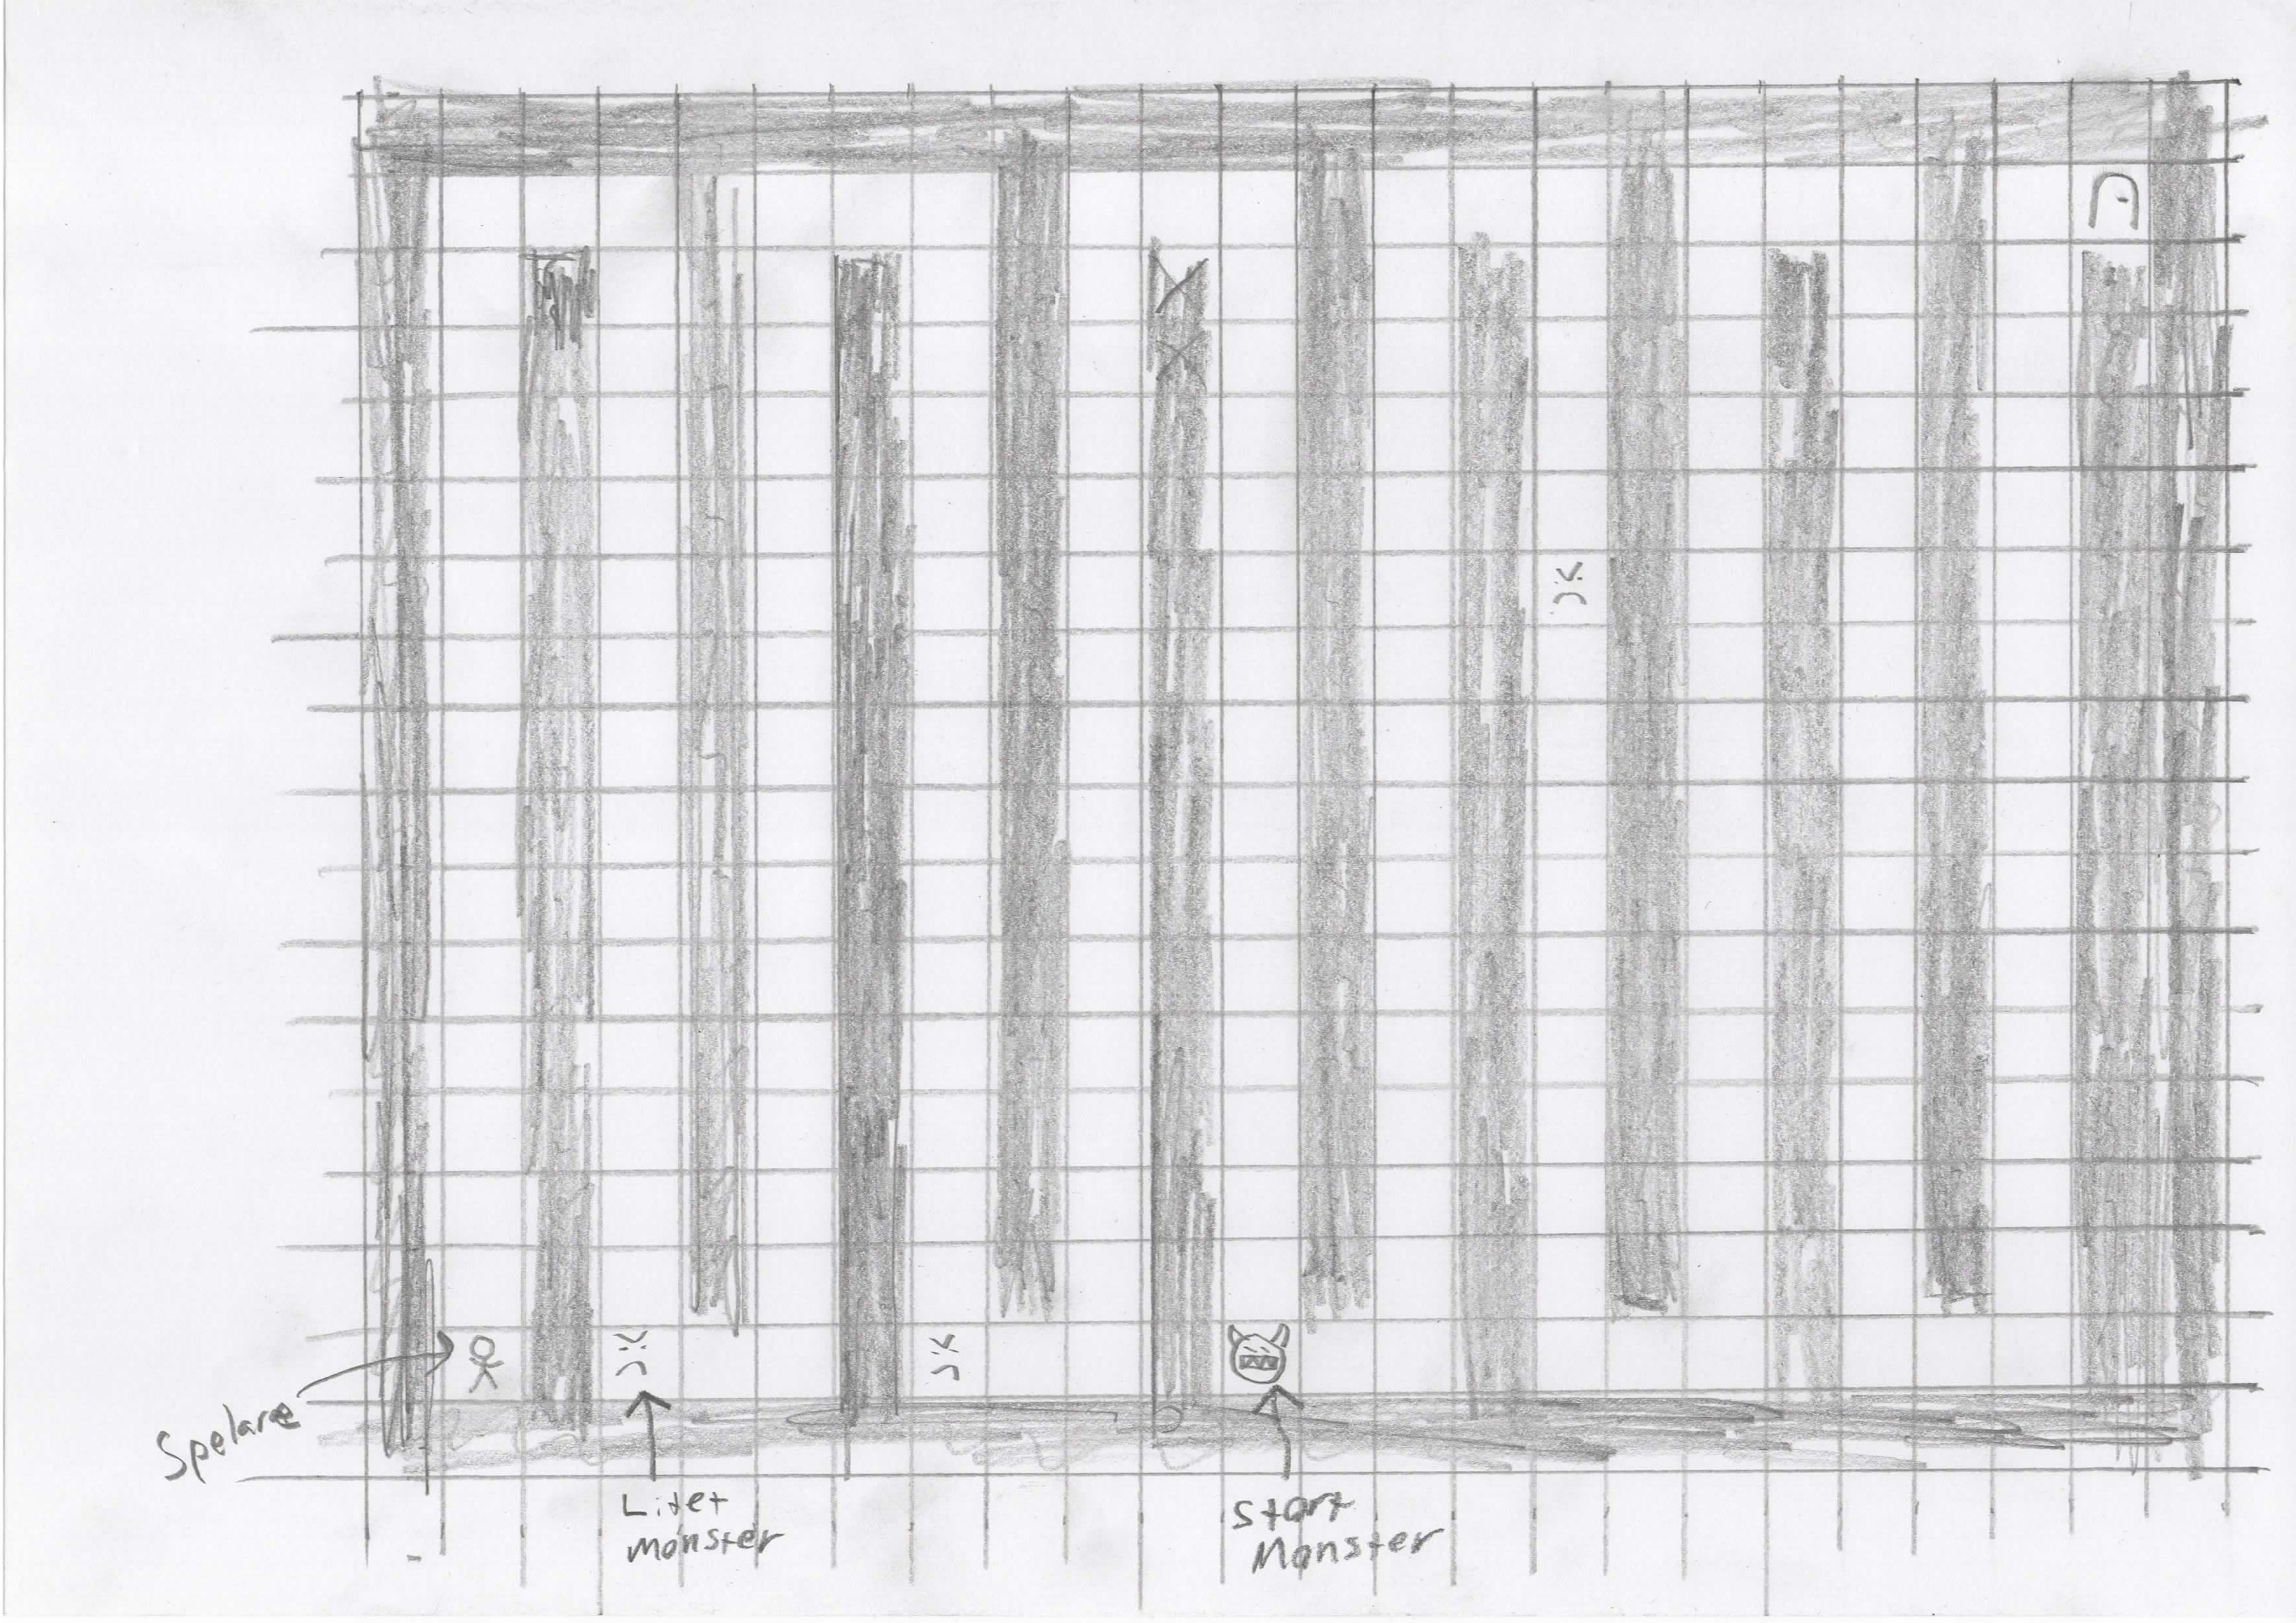
\includegraphics[scale=0.5]{Spelskiss}

\newpage
\section{Kravformulering}
\subsection{Ska-krav}
\begin{enumerate}
  \item Hela spelplanen ska synas i spelfönstret.
  \item Spelplanen ska vara en labyrint som är tvådimensionell och har väggar som så det blir en bana från start till slutpunkt.
  \item Väggar ska finnas på vissa positioner.
  \item Spelaren ska kunna röra sig åt fyra håll med hjälp av W, A, S och D.
  \item Spelaren ska ha ett antal livspoäng.
  \item Varken spelaren eller fienderna ska inte kunna gå igenom en vägg.
  \item När spelaren trycker på mellanslag ska spelaren attackera.
  \item Om en fiende är framför spelaren, inom attackavstånd och spelaren attackerar så ska fienden ta skada.
  \item Fiender ska röra positioner enligt en fördefinerad bana.
  \item Fienderna ska ha ett antal livspoäng.
  \item När en fiende har noll livspoäng så blir den fienden förintad.
  \item Fiender ska skada spelaren när de kolliderar.
  \item Spelaren ska tappa livspoäng när spelaren blir skadad.
  \item När spelaren har noll livspoäng ska spelet börja om.
  \item 2 typer av fiender ska finnas, en stor och en liten. Dessa ska göra olika skada och ska ha olika mycket liv. De ska ha olika rörelsemönster.
  \item Det ska finnas en utgång.
  \item Om spelaren koliderar med utgången ska nästa bana påbörjas.
  \item Slutpoängen ska räknas ut baserat på antalet förintade fiender och tiden det tar att klara spelet.
  \item Banorna ska skapas baserat på en textfil som specificerar var väggarna ska vara, vart utgången är och var 
\end{enumerate}

\subsection{Bör-krav}
\begin{enumerate}
  \item Fiender ska ha en chans att släppa ett liv när de förintas.
  \item Spelare ska kunna plocka upp liv för att fylla på sin hälsa.
  \item Fienderna ska röra sig mot spelaren när spelaren är inom synhåll.
  \item Det ska finnas "Powerups" på spelplanen som spelaren ska kunna plocka upp. Dessa powerups ska ge en positiv effekt till spelaren.
\end{enumerate}

\newpage
\section{Kravuppfyllelse}


\textbf{Spelet ska simulera en värld som innehåller olika typer av objekt. Objekten ska ha olika beteenden och röra sig i världen och agera på olika sätt när de möter andra objekt.}

Uppfylls av krav 1, 2, 4, 6, 8, 9, 12 och 17.

\textbf{Det måste finnas minst tre olika typer av objekt och det ska finnas flera instanser av minst två av dessa. T.ex ett spelarobjekt och många instanser av två olika slags fiendeobjekt.}

Uppfylls av krav 3, 4 och 15.

\textbf{Ett beteende som måste finnas med är att figurerna ska röra sig över skärmen. Rörelsen kan följa ett mönster och/eller vara slumpmässig. Minst ett objekt, utöver spelaren ska ha någon typ av rörelse.}

Uppfylls av krav 4 och 9
Både spelaren och båda fienderna kommer röra sig över spelplanen.

\textbf{En figur ska styras av spelaren, antingen med tangentbordet eller med musen. Du kan även göra ett spel där man spelar två stycken genom att dela på tangentbordet (varje spelare använder olika tangenter). Då styr man var sin figur.}

Uppfylls av krav 4 och 7. 
Spelaren styrs av W, A, S och D tangenterna och kan attackera med mellanslag.

\textbf{Grafiken ska vara tvådimensionell.}

Uppfylls av krav 2.
Grafiken kommer vara tvådimensionell 

\textbf{Världen (spelplanen) kan antas vara lika stor som fönstret (du kan göra en större spelplan med scrollning, men det blir lite krångligare).}

Uppfylls av krav 1, 2 och 17.
Labyrinten kommer fylla fönstret, när nästa bana påbörjas så kommer den nya labyrinten att ersätta den den gamla.

\textbf{Det ska finnas kollisionshantering, det vill säga, det ska hända olika saker när objekten möter varandra, de ska påverka varandra på något sätt. T.ex kan ett av objekten tas bort, eller så kan objekten förvandlas på något sätt, eller så kan ett nytt objekt skapas. (Ett exempel på att skapa/ta bort objekt är när man i Space Invaders trycker på skjuta-knappen, t.ex en musknapp, då avfyras ett laserskott och skottet blir då en ny figur som skapas och placeras i världen, på en position vid laserkanonens mynning. Skottet rör sig framåt (uppåt) och om det träffar ett fiendeskepp tas både skottet och skeppet bort, om skottet kommer utanför spelplanen, dvs det missar, tas det endast bort.)}

Uppfylls av krav 6 och 12. 
Spelaren kommer ta skada om den koliderar med en fiende.

\textbf{Det ska vara enkelt att lägga till eller ändra banor i spelet. Detta kan exempelvis lösas genom att läsa in banor från en fil (lite som i Sokoban-labben i TDP002), eller genom att ha funktioner i programkoden som bygger upp en datastruktur som definierar en bana.}

Uppfylls av krav 19.




\end{document}
